\documentclass[a4paper,10pt]{article}
\usepackage[margin=2.5cm]{geometry}
\usepackage[utf8]{inputenc}
\usepackage[colorlinks=true,urlcolor=blue]{hyperref}
\usepackage{amsmath}
\usepackage{graphicx}
\usepackage{float}
\usepackage{caption}
\usepackage{subcaption}

%\usepackage{listings} %Alternative to minted
\usepackage{minted}



\setlength{\parindent}{0em}
\setlength{\parskip}{1em}

\title{\textbf{1RT730 Project Report} 
	\\ CLIMES(Climate-Induced Medical Emergency System)-Monitor}
\author{Jianyu Liu, Rui Ma, Upali Bera}
\date{\today}

\begin{document}
	
\maketitle
    
 \section{Introduction}
Our group project designs and analyzes a real-world LLM solution to monitor climate-induced public health vulnerabilities in Uppsala County. Uppsala is where we study, and due to climate change Europe has experienced severe heatwaves that caused substantial excess mortality\cite{henley2026excess}. Although these events may appear distant, they already affect Uppsala residents and create local risks\cite{uppsala_klimatanpassning}. Residents and international students currently lack an accessible channel that combines live local observations with historically grounded heat frequencies and source-supported preparedness guidance without inventing numbers or medical advice. CLIMES-Monitor addresses this gap with a guardrail-first architecture whose main contributions are (1) deterministic historical-frequency calculation from the SMHI series, (2) neighbourhood-level weather retrieval, and (3) constrained passage selection from Swedish and secondary manuals.

\section{Dataset}
\subsection{OpenStreetMap}
For this project, we need detailed geographical information in Uppsala\cite{openstreetmap_uppsala}, so we chose OpenStreetMap in the Uppsala Area and extracted a 126MB XML file, which contains around 2800 buildings/roads/etc. in Uppsala. Then we extracted the building and community names from the XML and output JSON files for location resolution. The challenge is to identify the file structure and process it correctly.
\subsection{WeatherMetro}
Then, a real-time weather source is needed, so we used the WeatherMetro API, which provides current and forecast information in a certain area using coordinates matched to named communities (e.g., Flogsta). The size is pretty big(hard to estimate) and the type is a JSON file. To process it, we need to get access to the API and provide the name of the place; some useful information will be returned. The challenges are that they require exact strings, so for some communities with Swedish characters(e.g., Gränby), it is hard to search.


\subsection{SMHI}
Historical temperature data come from the SMHI Open Data Meteorological Observations API (parameter 20, daily maximum temperature) at station 97510 (Uppsala Aut). 
The series contains 15\,004 quality-controlled daily values from 1 June 1985 to 30 June 2026 (approximately 41 years). 
After skipping metadata rows and parsing dates we extracted consecutive-day heatwave runs using thresholds aligned with Swedish practice: $\ge 27^\circ$C for at least three days, $\ge 30^\circ$C for at least three days, $\ge 25^\circ$C for at least five days, and single-day maxima $\ge 33^\circ$C. 
The long record required careful handling of quality codes and missing days; absolute thresholds were chosen for a cool Nordic climate rather than southern-European definitions. 
Official national observations provide a free, continuous baseline for any Uppsala-specific heat-health analysis.

\subsection{Knowledge base}
To support preparedness answers we built a local retrieval store from three groups of documents. 
Swedish civil-protection guidance from Myndigheten för civilt försvar (MCF) supplies the most authoritative local advice; six PDFs (about 4\,MB) were selected\cite{mcf_naturolyckor}. 
The content is in Swedish, so the model may occasionally retain Swedish phrasing or produce imperfect translations, but these sources remain the most relevant for Uppsala conditions. 
We also included the climes policy brief \textit{Healthcare preparedness in a changing climate}\cite{climes_healthcare}, which addresses healthcare-system vulnerabilities under climate extremes in a Swedish context. 
A smaller secondary set of U.S.\ FEMA severe-weather leaflets (four PDFs, about 1\,MB)\cite{ready_severe_weather} is retained for general tips; their main limitation is the U.S.\ context, which is less suitable for Swedish housing, climate and health-system conditions. 
All documents were processed with \texttt{pypdf} and LangChain, chunked, and indexed with \texttt{all-MiniLM-L6-v2} embeddings into a persistent Chroma store so that preparedness answers can cite concrete passages rather than free-form medical claims.


\subsection{Prompt Engineering}
The final system combines deterministic rules with a constrained LLM prompt. Rules handle request routing, location matching, weather-data validation, and rejection of unrelated requests. Current weather and forecast responses are rendered directly from validated tool output, reducing the risk of invented values or unsupported interpretations.

For preparedness questions, the prompt instructs Qwen3.5-2B to select one or two relevant passage identifiers from the retrieved context and return them in a strict JSON format. The application validates this selection and presents complete source-supported sentences with concise source references rather than allowing the model to freely rewrite safety advice. If the selection is invalid, a retrieval-based fallback is used. Hypothetical scenarios are explicitly labelled and kept separate from actual observations and forecasts.


\section{Architecture}

CLIMES combines rule-based processing, external weather data, and retrieval-supported LLM passage selection. As shown in Figure 1, weather queries and preparedness questions follow separate paths. This separation helps distinguish observed conditions from general guidance and hypothetical scenarios. The heat thresholds used by the deterministic risk rules ($27\,^{\circ}\mathrm{C}$ and $30\,^{\circ}\mathrm{C}$) are fixed project-defined indicators, separate from the historical comparison. Explicit historical queries and hypothetical multi-day heat queries call a deterministic historical-comparison function based on the 41-year SMHI series, using the user's exact temperature and minimum duration. Matching run counts are calculated and rendered programmatically rather than generated by the language model; they describe past observations, not health risk or future probability.

\begin{figure}[htbp]
    \centering
    \IfFileExists{climes_architecture.png}{%
        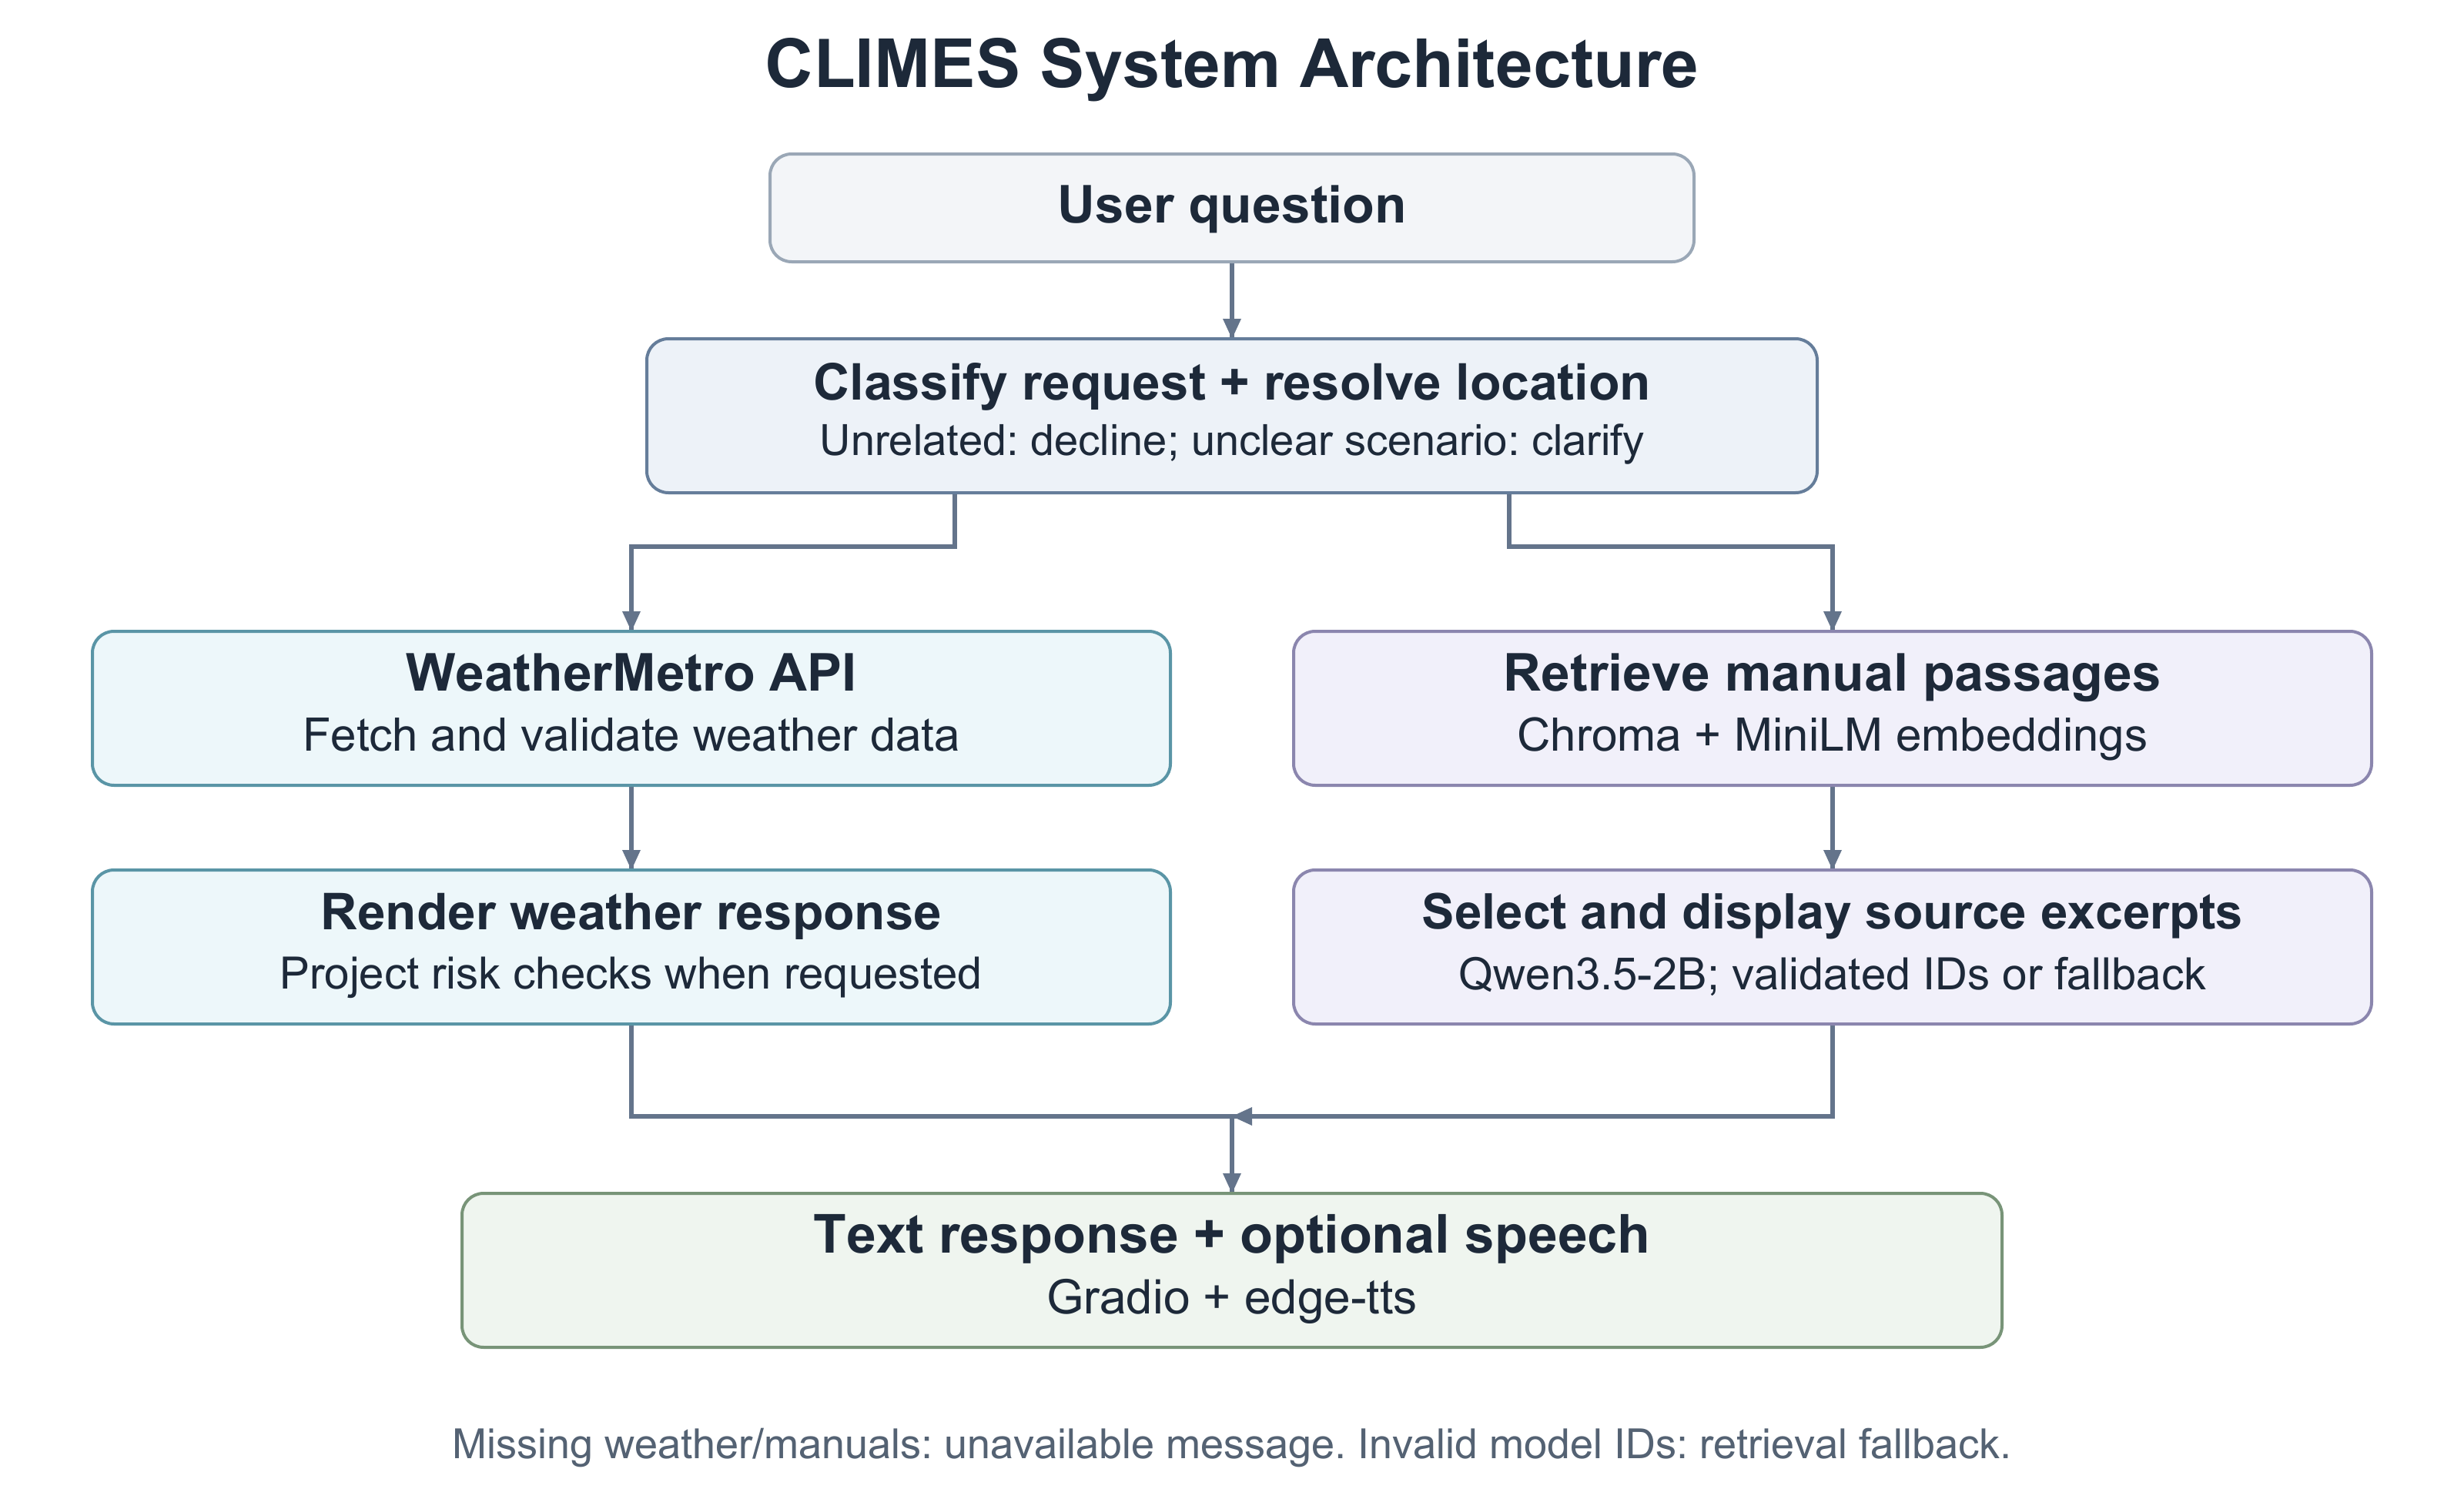
\includegraphics[width=\linewidth]{climes_architecture.png}%
    }{%
        \fbox{\parbox[c][3cm][c]{0.9\linewidth}{\centering
        \texttt{climes\_architecture.png}\\[6pt]
        Image available in the original report project.}}%
    }
    \caption{Simplified architecture of CLIMES. Weather responses use validated tool data, while preparedness responses present concise source-supported guidance. The historical-comparison path is omitted from this simplified diagram: explicit historical queries use the SMHI comparison tool directly, and hypothetical multi-day heat queries combine preparedness guidance with the historical comparison.}
    \label{fig:climes-architecture}
\end{figure}

\subsection*{3.1 Request routing and weather processing}
Deterministic rules classify requests and match location names against a local place dictionary. Unicode normalisation and case-insensitive matching support Swedish names, while specific neighbourhoods take priority over the city. Weather queries use the resolved coordinates to request current observations or forecasts from WeatherMetro. Required fields are validated before direct rendering; missing or invalid data produce an explicit unavailable response. Forecast dates are selected using the Europe/Stockholm date. Current risk-status queries additionally apply project-defined thresholds, which are explicitly distinguished from official weather warnings.


\subsection*{3.2 Retrieval and LLM passage selection}
Preparedness questions retrieve passages from a persistent Chroma vector store using all-MiniLM-L6-v2 embeddings. Topic- and audience-based filtering selects the designated English heat, winter-storm, or flood leaflet for residents, or the CLIMES brief for healthcare questions. Passages are deduplicated, and source-specific unit clarifications are applied. The base Qwen3.5-2B model selects one or two passage identifiers in a strict JSON format. The application validates these identifiers and uses a retrieval-based fallback if the selection is invalid. Complete selected sentences are presented as concise guidance with source labels, limiting unsupported rewriting of safety information. Hypothetical temperatures remain user assumptions and do not trigger actual weather retrieval.

\subsection*{3.3 Interface and speech output}
The Gradio interface displays the text response before generating optional speech through edge-tts. Speech-service failures leave the text available. Execution logs record routing, tool results, retrieval, passage selection, responses, and audio outcomes to support evaluation and debugging.

\section{Results}
We evaluated CLIMES-Monitor through predefined prompt tests, fault injection, and targeted browser checks. The following sections report quantitative measurements, representative outputs, strengths, and limitations. Automated checks and
manual observations are distinguished because passing a structural check does not necessarily establish complete task success. 

\subsection{Quantitative results}
We evaluated CLIMES-Monitor using 15 predefined English prompts covering current weather, forecasts, two Uppsala neighbourhoods, preparedness advice, hypothetical conditions, false premises, unrelated requests, healthcare guidance and historical comparisons. Testing used Qwen3.5-2B on a Google Colab Tesla T4. Weather responses were compared with the same-turn tool output, while preparedness responses were checked against the retrieved passages. Two additional fault-injection tests simulated a timeout and incomplete weather fields.

\begin{table}[htbp]
\centering
\small
\renewcommand{\arraystretch}{1.15}
\begin{tabular}{@{}p{0.28\linewidth}p{0.68\linewidth}@{}}
\hline
\textbf{Evaluation} & \textbf{Observed result} \\
\hline
Offline regression & 38 test methods passed, including the 16 original risk-rule boundaries. \\
Integration checks & 19 test methods passed. \\
Runtime structural checks & 15/15 predefined prompts passed the automated checks. \\
Simulated interface failures & 2/2 returned an explicit unavailable response without invented observations. \\
LLM passage selection & 6/6 returned valid selections; no retrieval fallback was required in this run. \\
Text completion latency & Median 0.62 s; mean 0.87 s; range 0.17--3.86 s across the 15 prompts. \\
\hline
\end{tabular}
\caption{Final batch results. Automated structural passes are not an overall accuracy estimate.}
\end{table}

The failures described below concern earlier development versions. The structural checks did not establish complete task success. Manual review found that the three-day forecast included today. A separate speech check failed in the notebook's asynchronous execution environment, and subsequent browser testing exposed an empty-reply issue in Gradio message preprocessing. After correction, targeted runtime and browser checks confirmed non-empty replies, generated and playable speech, and a three-day forecast starting tomorrow. These checks were recorded before the final batch above.

Latency was measured from submission to the first complete text response, excluding model loading, speech generation, and playback. Some requests used cached data. These timings describe the final batch. No controlled baseline-model comparison was conducted, so no comparative accuracy or speedup is claimed.


\subsection{Qualitative results}
\subsubsection{example outputs}
Figure~\ref{fig:flogsta-output} shows a response to a weather
query for Flogsta, Uppsala. The interface displays the
neighbourhood name, temperature, wind speed, relative humidity,
recorded precipitation, and observation timestamp.
The response identifies the weather-service tool as its source
and explicitly states that official weather warnings were not
checked. An audio player provides an additional way to access
the response. This example illustrates the revised interface
and output format rather than independently validating
weather accuracy or accessibility.

\begin{figure}[H]
    \centering
    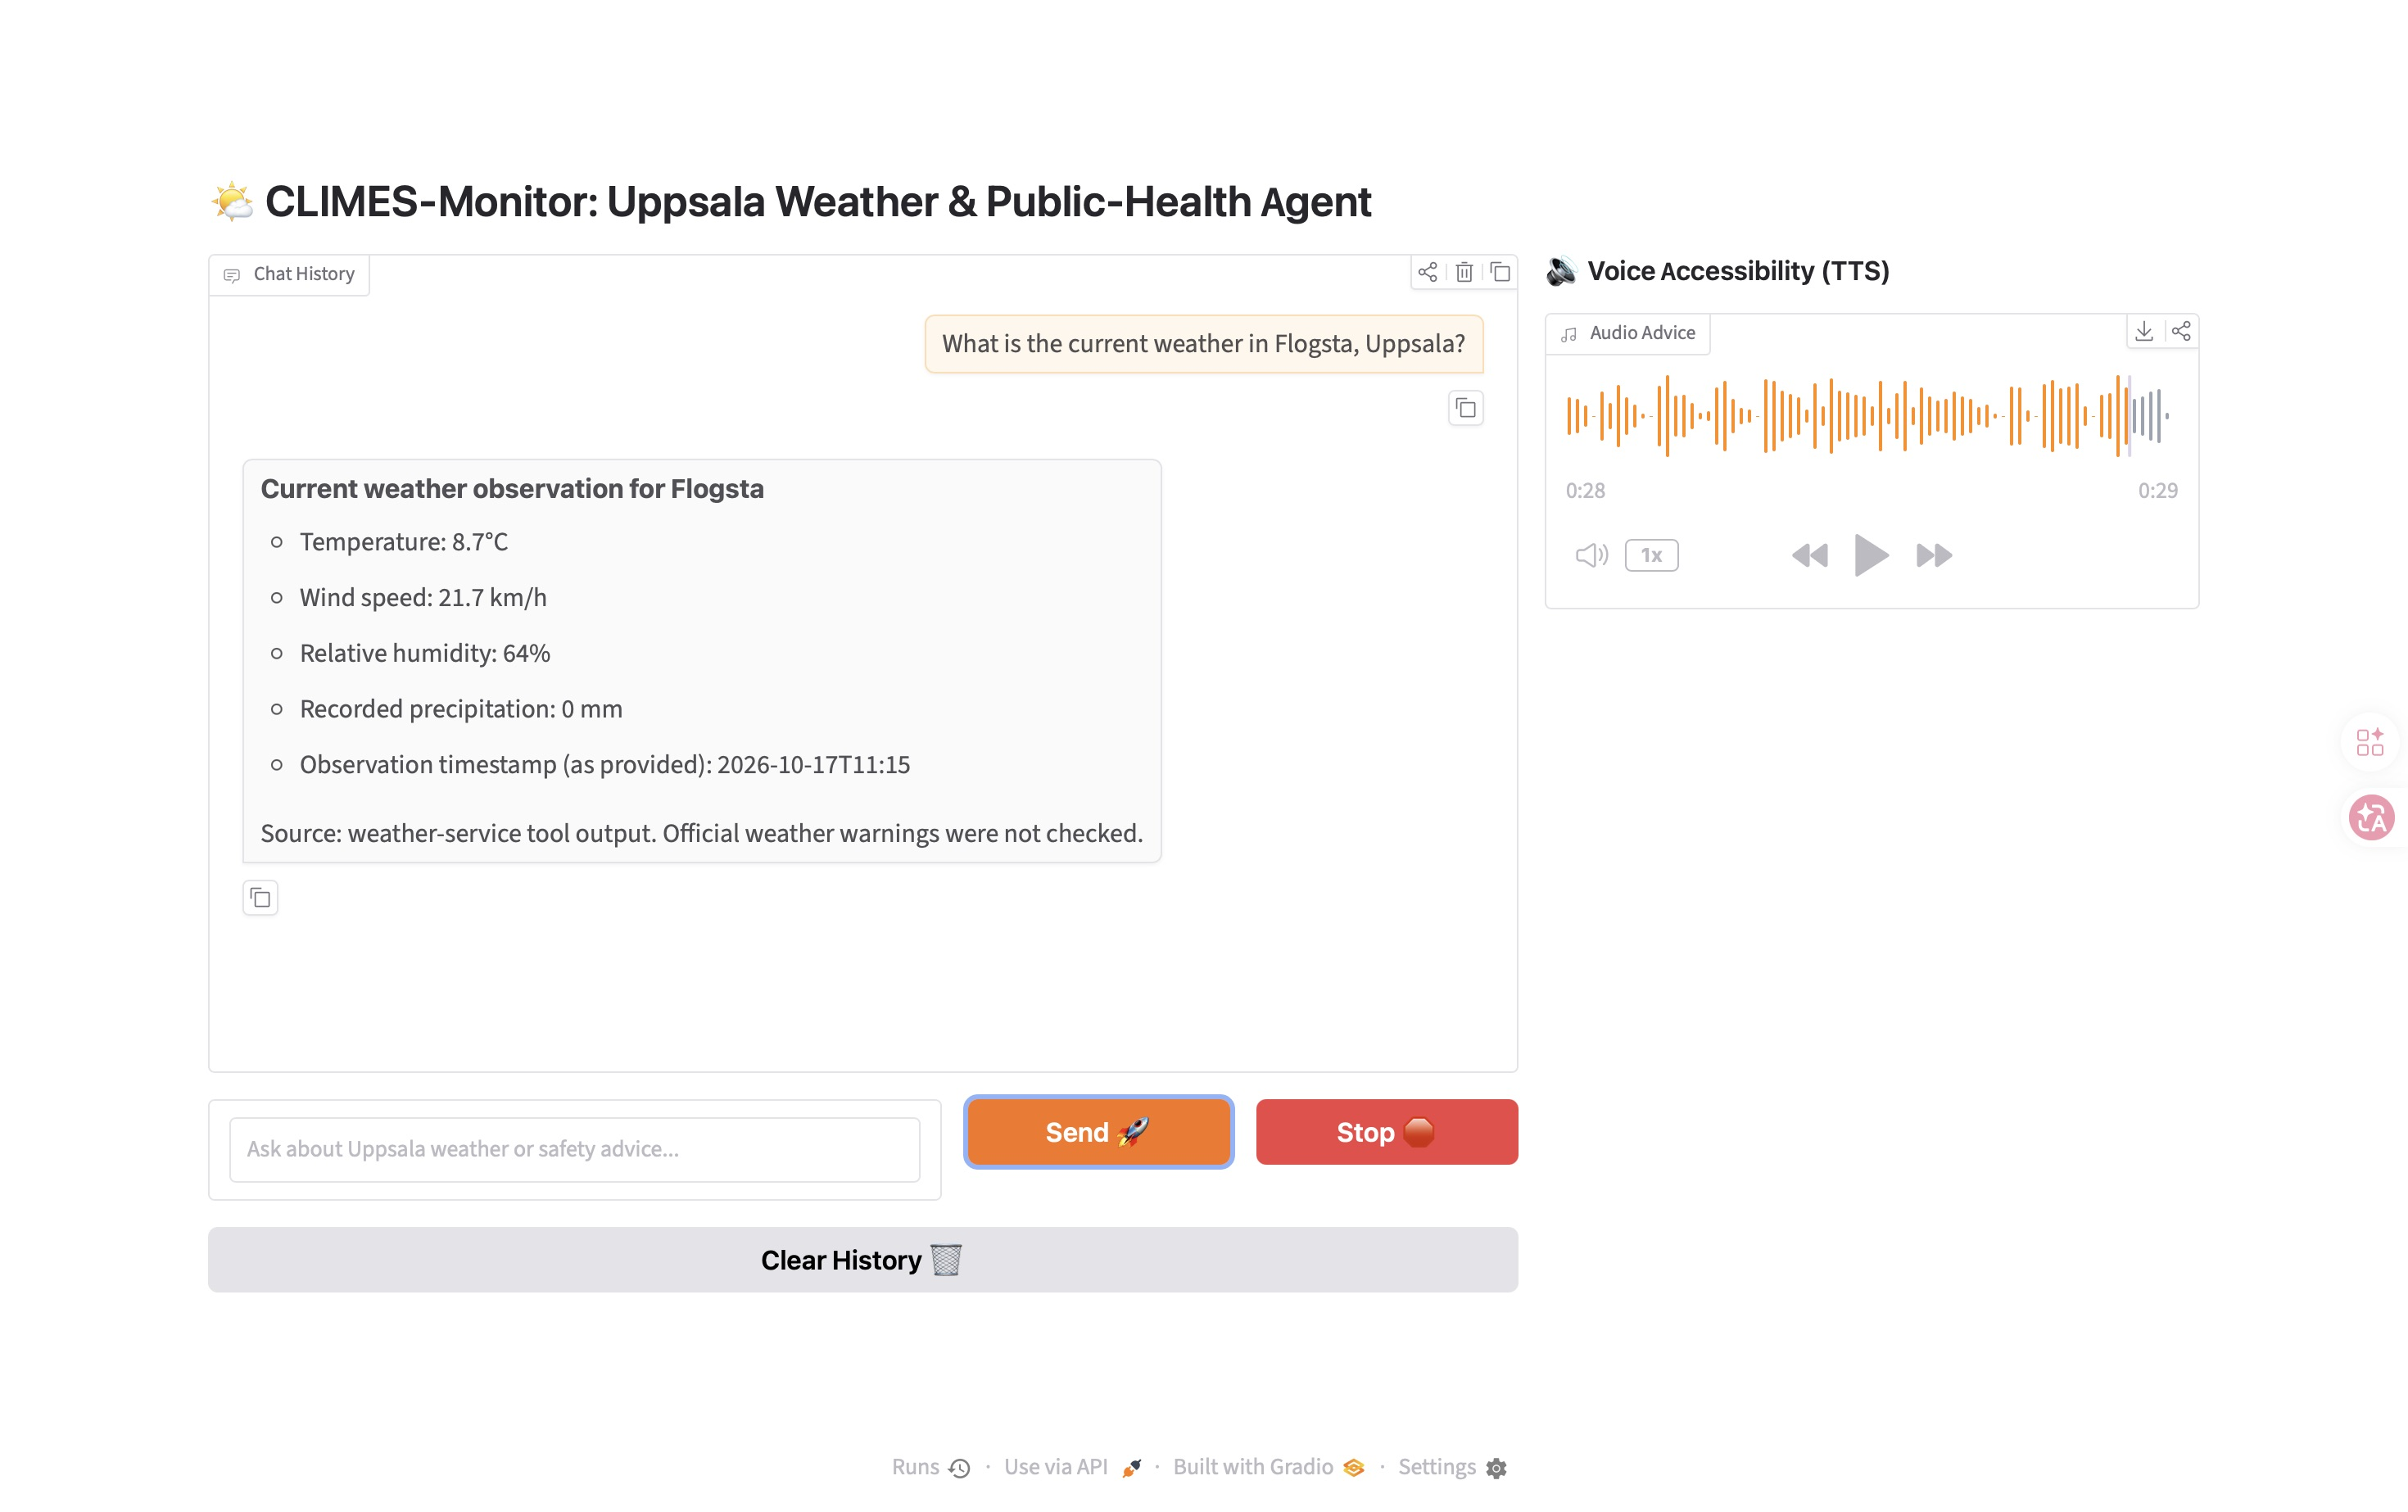
\includegraphics[width=0.90\linewidth]{flogsta.jpeg}
    \caption{A weather response for Flogsta in the revised
    CLIMES interface, with observation details and
    text-to-speech playback.}
    \label{fig:flogsta-output}
\end{figure}



%\subsubsection{user feedback}
%Informal testing within the group confirmed that live weather answers matched the tool output for the requested neighbourhood and that hypothetical multi-day heat queries returned historically grounded frequencies from the SMHI series rather than invented rates. 
%Preparedness questions retrieved Swedish and climes material when relevant. 
%No formal external user study was conducted before submission; systematic evaluation with Uppsala residents remains future work.

\section*{4.3 Strengths}
\begin{itemize}
\item \textbf{Grounded weather responses:} Current weather and forecast answers are rendered directly from validated tool output. Missing or invalid data produce an explicit unavailable response instead of invented observations.
\item \textbf{Neighbourhood resolution:} The system prioritises specific neighbourhood names over the city name. Tests confirmed that requests containing ``Flogsta, Uppsala'' and ``Gr\"anby, Uppsala'' resolve to the corresponding neighbourhood coordinates. This demonstrates location matching, although the spatial accuracy of the weather data was not independently evaluated.
\item \textbf{Traceable preparedness information:} Safety responses present complete source-supported sentences rather than freely generated medical advice. Constrained passage selection and a retrieval-based fallback help preserve the wording and units of the source material.
\item \textbf{Optional speech output:} The interface provides text-to-speech playback as an additional way to access responses. Playback was verified in browser testing, although usability for people with visual impairments has not yet been evaluated.
\end{itemize}


\subsection{Limitations}
The evaluation used a small, predefined English prompt set and one runtime configuration. It does not establish performance on arbitrary queries or real emergencies. All six model-selection calls returned valid selections in the final run, but this small sample does not establish general reliability. Responses use complete sentences, but coverage is limited by the retrieved material and approved sentence set. The resident guidance route uses selected English-language US manuals, whose applicability to Swedish conditions is limited; indexed Swedish documents are not evidence of coverage by this route. The system does not check an official warning feed, and its project thresholds do not establish a multi-day heatwave or flood risk. Dependence on external weather and speech services can affect availability. Clinical accuracy, improved emergency outcomes, and population-level accessibility were not evaluated. Context-dependent follow-up questions are not currently supported.

\section{Societal Impact}

CLIMES-Monitor improves access to location-specific weather and preparedness information for Uppsala residents and international students. 
By combining live observations with deterministic thresholds and retrieved official guidance, the system can help users recognise heat, cold, wind or heavy-rain conditions earlier and take simple protective actions. 
Neighbourhood-level resolution and optional speech output further support people who may not follow national forecasts closely.

The main risks are over-reliance and misinterpretation. 
Project-defined thresholds are not official SMHI warnings; treating them as such could create false alarm or false safety. 
Retrieved safety text still includes a limited amount of U.S.\ FEMA material whose context differs from Swedish conditions, although Swedish MCF guidance and the climes healthcare brief are now prioritised. 
Any residual model error, incomplete weather data, or speech-service failure could produce incomplete or misleading answers. 
Privacy exposure is limited because no personal health data are stored, but location queries still reveal user interest in specific neighbourhoods.

We mitigate these risks by rendering current weather and forecasts directly from validated tool output rather than free generation, by displaying source excerpts for preparedness advice instead of rewritten medical claims, by explicitly labelling hypothetical scenarios, and by logging routing and tool results for inspection. 
The system is intended as a decision-support aid, not an emergency service; users are directed to official channels when real warnings are needed. 
Future work should further reduce reliance on non-Swedish leaflets and evaluate the tool with local users.

\hfill \break
\textit{\textbf{Use of generative AI}}

Rui: I used OpenAI Codex to assist with debugging and revising the application code. I also used it to create the architecture diagram.

Jianyu: I used Google Gemini to help me debug and set up the system environment, and to generate \texttt{bibitem}.

Upali: Used to assist with exploratory data analysis of the SMHI series, design of the heatwave definitions and historical-frequency tool, integration of the climes policy brief into the RAG knowledge base, and drafting of report sections on data and societal impact.

%\hfill \break
%\textit{\textbf{Note}}

%Report should be max. 4-6 pages long.

	
\begin{thebibliography}{50}

\bibitem{henley2026excess}
Henley, J. (2026, August 25). 
\textit{At least 35,000 excess deaths recorded in Europe's back-to-back heatwaves}. 
The Guardian. 
\url{https://www.theguardian.com/environment/2026/aug/25/at-least-35000-excess-deaths-europe-back-to-back-heatwaves}

\bibitem{uppsala_klimatanpassning}
Uppsala kommun. (n.d.). 
\textit{Klimatanpassning}. 
Retrieved October 15, 2026, from \url{https://www.uppsala.se/klimatanpassning}

\bibitem{openstreetmap_uppsala}
OpenStreetMap contributors. (2026). 
\textit{Map of Uppsala, Sweden} [Map]. 
Retrieved October 15, 2026, from \url{https://www.openstreetmap.org/export#map=12/59.8388/17.6538}

\bibitem{ready_severe_weather}
Ready.gov. (n.d.). 
\textit{Severe Weather}. 
Official website of the Department of Homeland Security. 
Retrieved October 15, 2026, from \url{https://www.ready.gov/severe-weather}

\bibitem{mcf_naturolyckor}
Myndigheten för civilt försvar (MCF). (n.d.). 
\textit{Naturolyckor och klimat}. 
Retrieved October 15, 2026, from \url{https://www.mcf.se/sv/amnesomraden/skydd-mot-olyckor-och-farliga-amnen/naturolyckor-och-klimat/}

\bibitem{climes_healthcare}
Centre for Impacts of Climate Extremes (CLIMES). (n.d.). 
\textit{Healthcare preparedness in a changing climate} [Policy brief]. 
Uppsala University / CLIMES. 
Retrieved October 2026 from \url{https://www.climes.se/outreach/policybriefs/}
		
\end{thebibliography}

	
	
%	\pagebreak
%	
%	\appendix
%	\section{Code}
%	\label{app:code}
%	
%	\inputminted[frame=lines,framesep=2mm,linenos]{python}{your_code.py}
%	
\end{document}
